\documentclass[12pt]{article}
% Required Packages
\usepackage[utf8]{inputenc}
\usepackage{geometry}
\geometry{letterpaper, margin=1in}
\usepackage{subcaption}
\usepackage{amsmath}
\usepackage{graphicx}
\usepackage{booktabs}
\usepackage[numbers,super]{natbib} % For ACS citation style baseline
\usepackage{hyperref}
\usepackage{fontawesome5} % for using icons
\usepackage[dvipsnames]{xcolor}
\usepackage{textcomp}
\usepackage{pdfpages}
\usepackage{siunitx}
\usepackage{adjustbox}

\begin{document}

\begin{center}
    \Large \textbf{Lab \#4: Vibrational-Rotational Spectra of Diatomic Molecules}
\end{center}
\vspace{0.5em}
\noindent
\begin{minipage}[t]{0.5\textwidth}
    \small
    \textbf{Name:} Yuchen Shi \\
    \textbf{Lab Partner:} Yizhe Dai, Siqi Li \\ 
    \textbf{Section:} 001
\end{minipage}%
\begin{minipage}[t]{0.5\textwidth}
    \small \raggedleft
    \textbf{Date Performed:} 2026-03-10 \\ 
    \textbf{Date Submitted:} 2026-03-24  
\end{minipage}
\vspace{1.5em}

\begin{abstract}
\noindent
The rovibrational spectra of HCl and DCl were recorded with an FTIR spectrometer in advance and analyzed to obtain rotational, vibrational, and structural constants. Assigned P-branch and R-branch lines were used in linearized forms of the rovibrational equations to determine \(B_0\), \(B_1\), \(D_e\), and the band origin. The values were combined with literature overtones and higher-\(v\) rotational constants to obtain \(B_e\), \(\alpha_e\), \(\tilde{\nu}_0\), and \(\tilde{\nu}_0\chi_e\). The final results were \(B_e=10.58441 \pm 0.00225\) and \(5.44881\pm0.00067\ \mathrm{cm^{-1}}\) for H\(^{35}\)Cl and D\(^{35}\)Cl, respectively; \(r_e=1.27509\pm0.00014\) and \(1.27458\pm0.00008\ \text{Ang}\); and \(k=551.87366 \pm 0.06886\) and \(541.83065 \pm 0.03540\ \mathrm{N\,m^{-1}}\). The bond lengths agreed closely with literature values with overall errors below 0.05\%, while the force constants have slightly higher error rates of 5 to 7\%.
\end{abstract}


\section*{Introduction}

The purpose of this experiment is to analyze the vibration-rotation spectra of \(\mathrm{H}^{35}\mathrm{Cl}\) and \(\mathrm{D}^{35}\mathrm{Cl}\) using FTIR spectroscopy and to extract molecular constants from the experimental data. In a diatomic molecule, infrared absorption excites both vibrational and rotational motion, producing a spectrum split into a \(P\)-branch and an \(R\)-branch around an unobserved central gap. In this experiment, the spectrum peaks of \({}^{35}\mathrm{Cl}\) were assigned and used to determine rotational constants, centrifugal distortion, vibrational constants, equilibrium bond lengths, and force constants.

For \(P\)-branch and \(R\)-branch transitions, combinations of peak positions linearize the rotational-vibrational expressions. The first relation,\cite{lab_manual}
\begin{equation}
\frac{\tilde{\nu}_R(J)-\tilde{\nu}_P(J)}{4(J+1/2)}
=
B_1-2D_e\left(J^2+J+1\right),
\end{equation}
was used to determine the rotational constant in the excited vibrational state, \(B_1\), from the intercept and the centrifugal distortion constant, \(D_e\), from the slope. 

A second linear combination,\cite{lab_manual}
\begin{equation}
\frac{\tilde{\nu}_R(J-1)-\tilde{\nu}_P(J+1)}{4(J+1/2)}
=
B_0-2D_e\left(J^2+J+1\right),
\end{equation}
gives the rotational constant in the ground vibrational state, \(B_0\), together with an independent estimate of \(D_e\). 

Finally, averaging an \(R\)-branch line with the neighboring \(P\)-branch line gives\cite{lab_manual}
\begin{equation}
\frac{\tilde{\nu}_R(J)+\tilde{\nu}_P(J+1)}{2}
=
\tilde{\nu}_{BO}+(B_1-B_0)(J+1)^2,
\end{equation}
where the intercept is the band origin \(\tilde{\nu}_{BO}\), which is the pure vibrational transition frequency, and the slope equals to \(B_1-B_0\). \cite{lab_manual}

To connect the measured \(v=0\) and \(v=1\) rotational constants with higher vibrational levels, the vibrational dependence of the rotational constant was described by \cite{lab_manual}
\begin{equation}
B_v = B_e-\alpha_e\left(v+\frac{1}{2}\right),
\end{equation}
where \(B_e\) is the equilibrium rotational constant and \(\alpha_e\) is the vibration-rotation interaction constant. Then, the experimentally determined \(B_0\) and \(B_1\) values were combined with literature values \cite{sime1990lit_all} to obtain \(B_e\) and \(\alpha_e\). Similarly, the vibrational term values were treated with\cite{lab_manual}
\begin{equation}
\frac{\tilde{\nu}_{B0}}{v'}
=
\tilde{\nu}_0-\tilde{\nu}_0\chi_e(v'+1),
\end{equation}
where the intercept gives the fundamental vibrational frequency \(\tilde{\nu}_0\) and the slope gives \(-\tilde{\nu}_0\chi_e\), with \(\chi_e\) as the first anharmonicity constant. 

Once \(B_e\) and the vibrational constants were obtained, structural and mechanical properties of the molecules could be calculated. The equilibrium bond length was determined from the rotational constant through \cite{lab_manual}
\begin{equation}
B_e=\frac{h}{8\pi^2 c \mu r_e^2},
\end{equation}
and the force constant was obtained from the harmonic vibrational frequency using\cite{lab_manual}
\begin{equation}
\tilde{\nu}_e=\frac{1}{2\pi c}\sqrt{\frac{k}{\mu}}.
\end{equation}
Overall, the rotational-vibrational spectrum provides a direct link between observed infrared transition frequencies and fundamental molecular properties such as bond length, anharmonicity, bond rigidity, etc.

\section*{Experimental}
Unfortunately the FTIR equipment is not available due to mechanical issues when this experiment was done and analysis was carried out with given spectrum, while the experimental and analysis method is given as below.

As for experiment, the FTIR spectrometer first warmed up for about 3 min. The acquisition parameters were set to 32 scans, a resolution of \SI{1}{cm^{-1}}, absorbance as the final format, and collection of a fresh background before each sample. The instructor would insert the gas cell, and spectra were recorded for the HCl and DCl samples.

As for analysis, the HCl spectrum was first displayed over \SIrange{3100}{2600}{cm^{-1}} and then examined in the narrower windows \SIrange{3100}{2890}{cm^{-1}} and \SIrange{2880}{2600}{cm^{-1}} for peak labeling. The DCl spectrum was displayed over \SIrange{2240}{1925}{cm^{-1}} and then labeled in the windows \SIrange{2220}{2090}{cm^{-1}} and \SIrange{2090}{1925}{cm^{-1}}. In both cases, only the stronger members of the doublets were analyzed, corresponding to H\(^{35}\)Cl and D\(^{35}\)Cl.

The measured wavenumbers were analyzed with linear regressions of specific equations in the manual \cite{lab_manual} to obtain slopes, intercepts, and their uncertainties in Python \cite{reback2020pandas,harris2020array,2020SciPy}. The values were combined with the higher-vibrational-state and overtone data from literature \cite{sime1990lit_all} to calculate \(B_e\), \(\alpha_e\), \(\tilde{\nu}_0\), and \(\tilde{\nu}_0\chi_e\). Finally, \(r_e\) and \(k\) were calculated from the fitted spectroscopic constants and compared with literature values \cite{herzberg2013bond_lit,lide2002constant_lit}.

\section*{Results}
The stronger peaks in each doublet peak were assigned to H\(^{35}\)Cl and D\(^{35}\)Cl. Eleven R-branch lines and ten P-branch lines were assigned for H\(^{35}\)Cl. Fourteen R-branch lines and thirteen P-branch lines were assigned for D\(^{35}\)Cl. The spectrum with assigned peaks are available in the Appendix and the raw splitting spectrum is presented here.

\begin{figure}[htbp]
    \centering
    \begin{subfigure}{0.48\textwidth}
        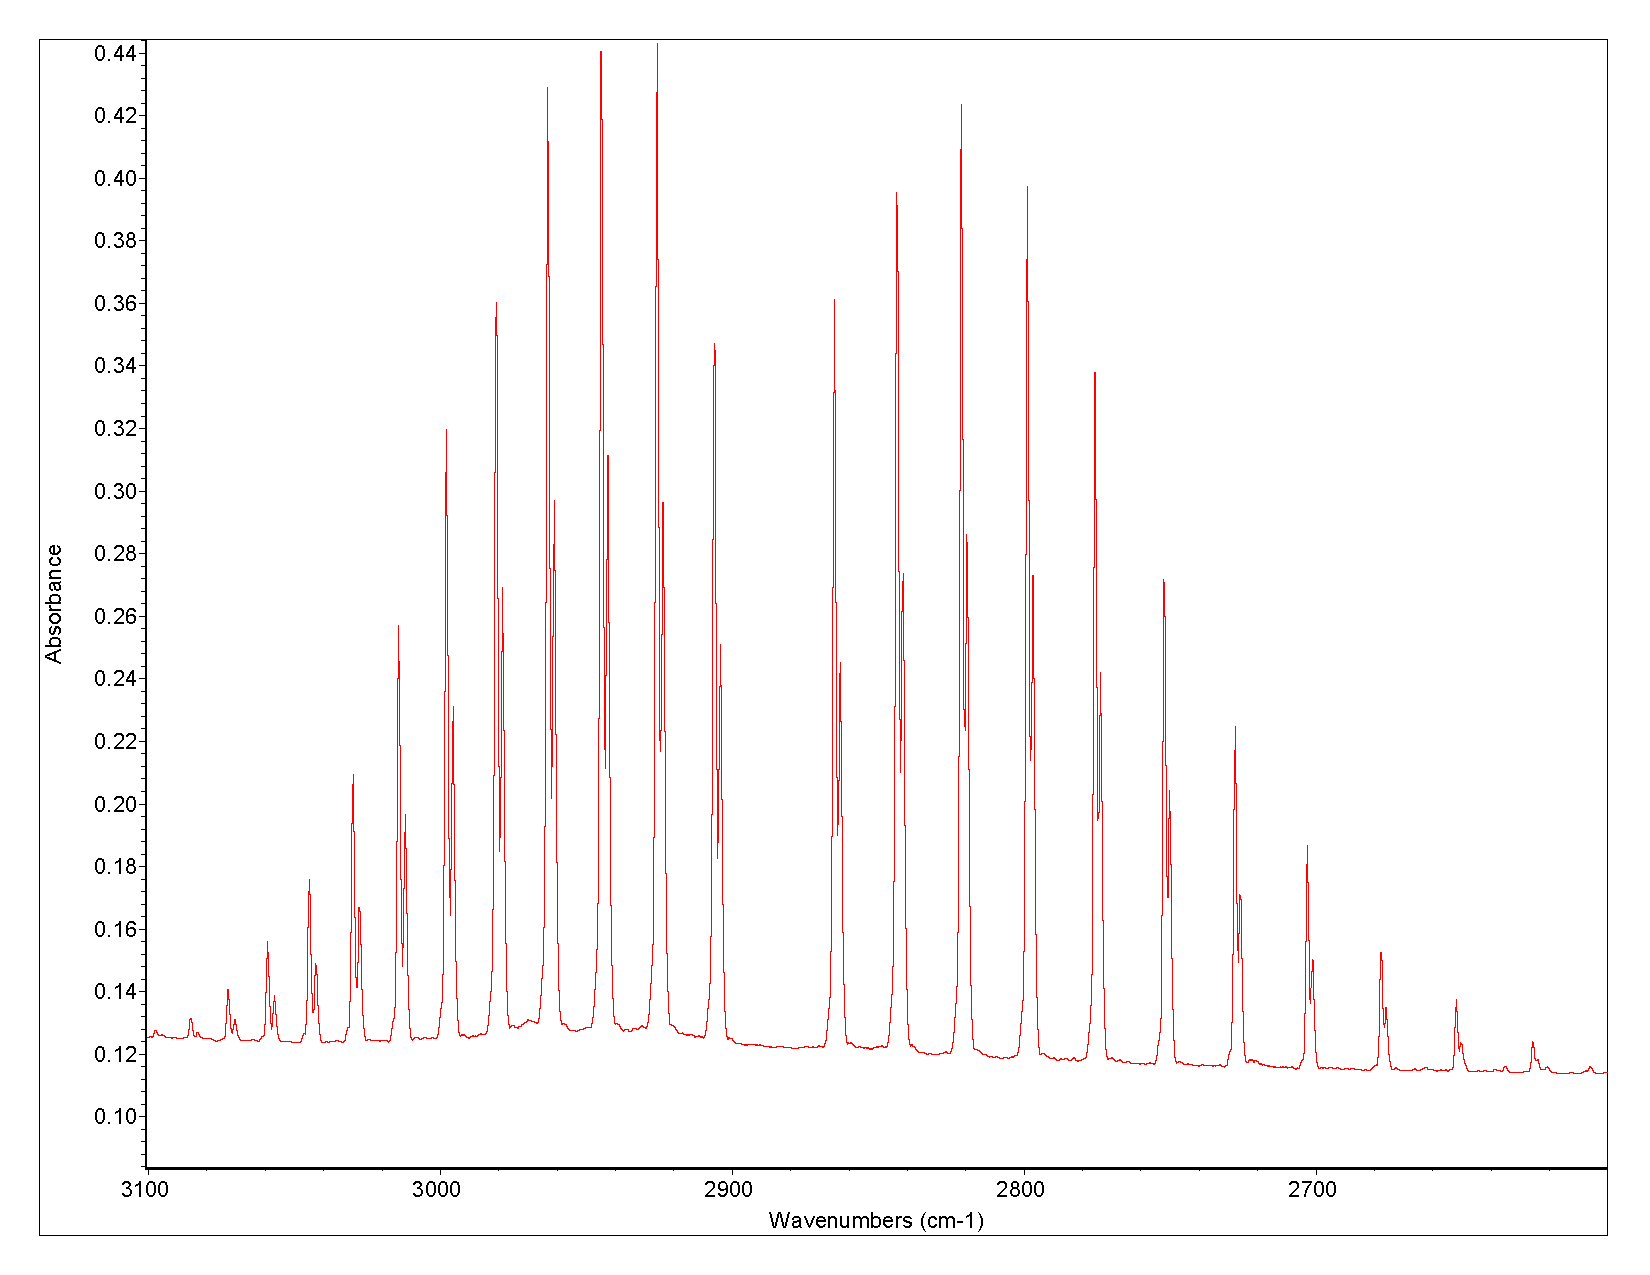
\includegraphics[width=\linewidth]{experimental_data/HCl_Entire.pdf}
        \caption{Entire Spectrum of H\(^{35}\)Cl}
    \end{subfigure}
    \hfill
    \begin{subfigure}{0.48\textwidth}
        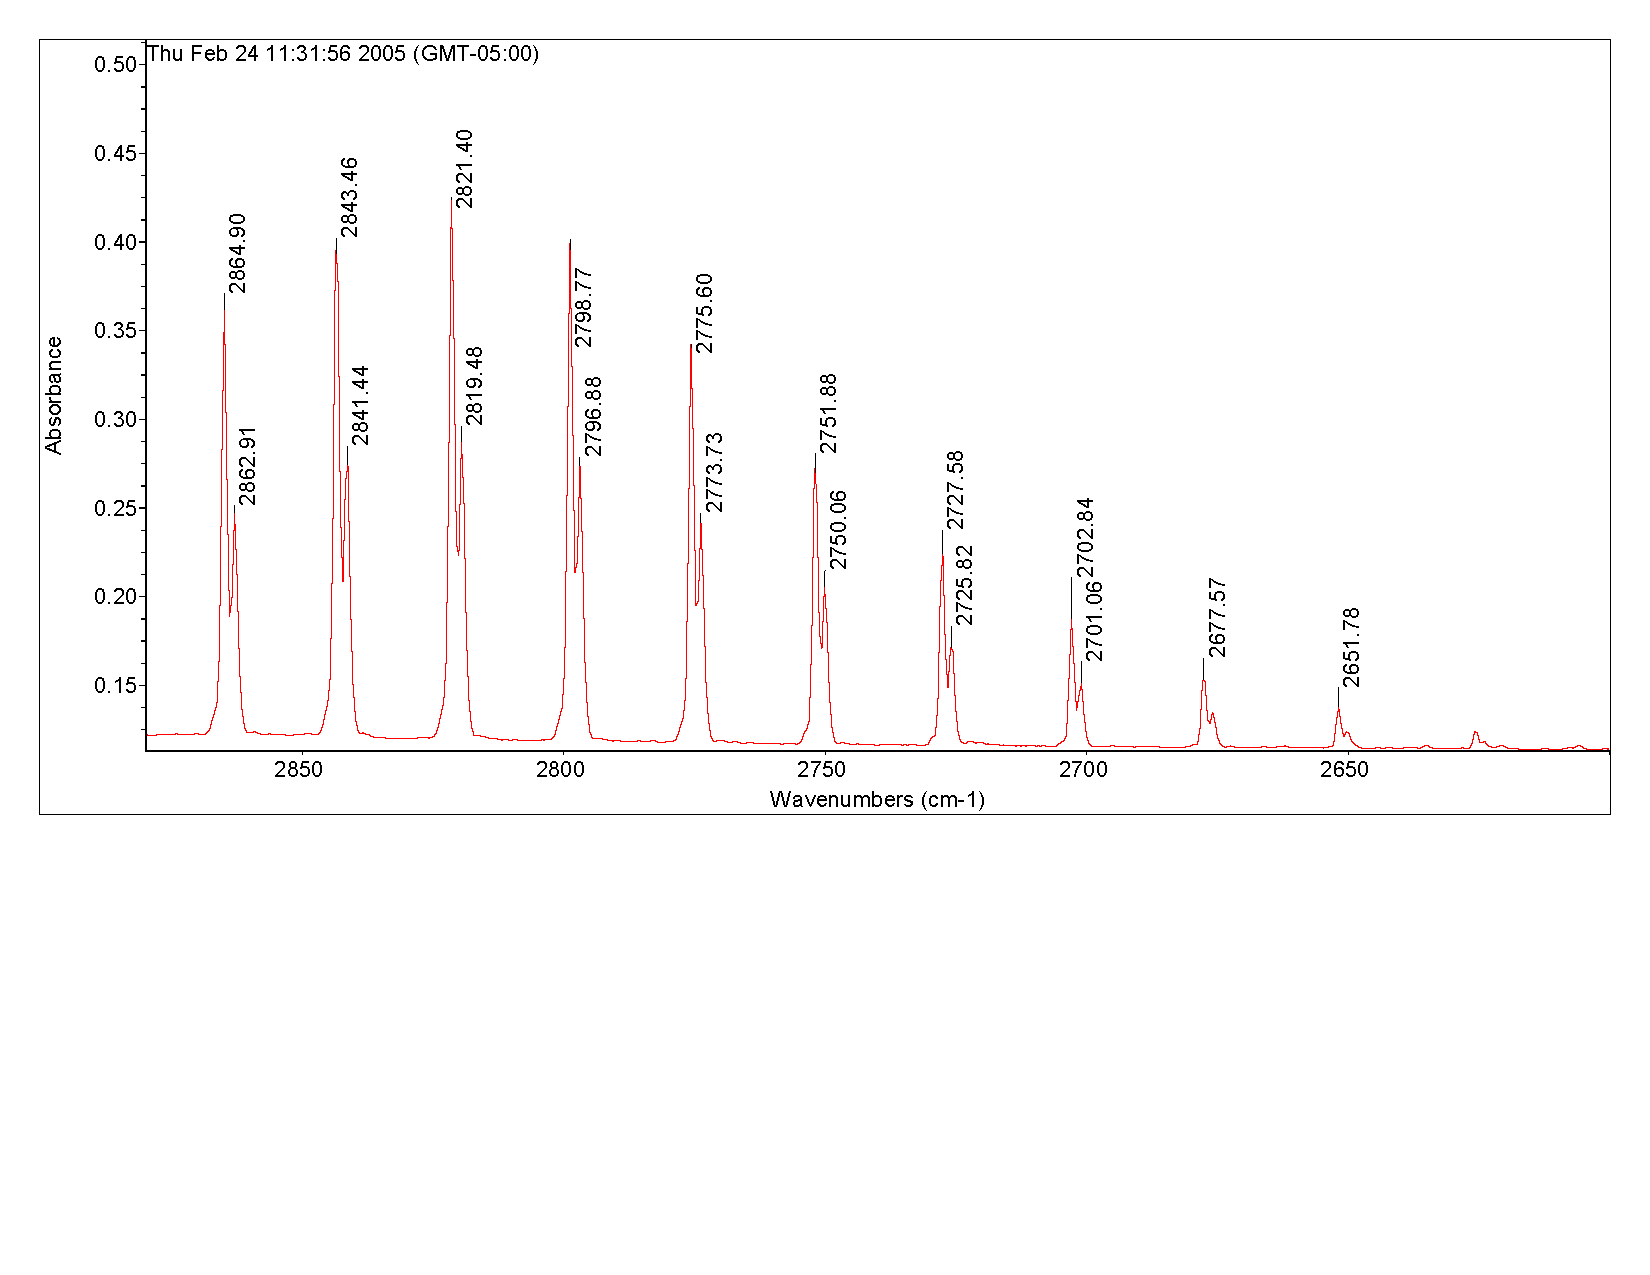
\includegraphics[width=\linewidth]{experimental_data/HCl_Right_clean.pdf}
        \caption{P-branch of H\(^{35}\)Cl}
    \end{subfigure}
    \hfill
    \begin{subfigure}{0.48\textwidth}
        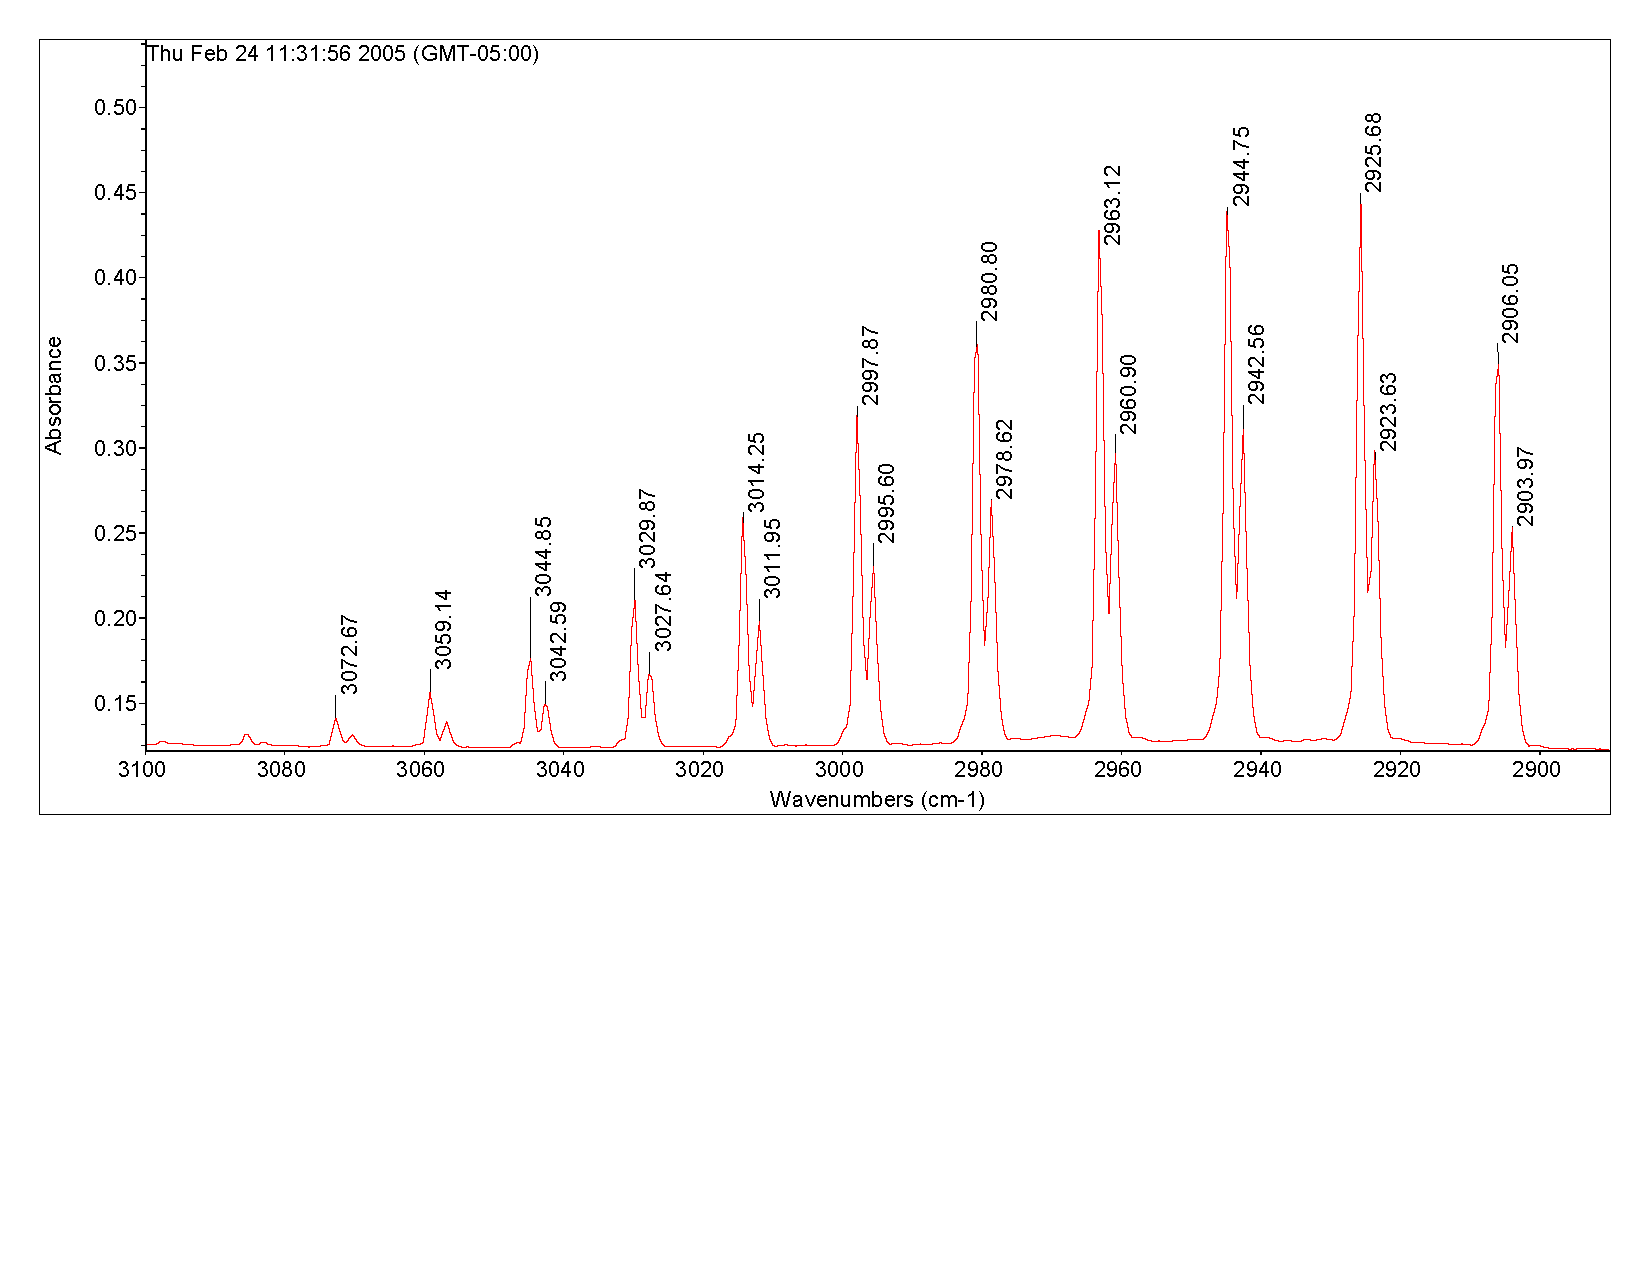
\includegraphics[width=\linewidth]{experimental_data/HCl_Left_clean.pdf}
        \caption{R-branch of H\(^{35}\)Cl}
    \end{subfigure}
    \caption{IR spectrum of H\(^{35}\)Cl.}
\end{figure}

\begin{figure}[htbp]
    \centering
    \begin{subfigure}{0.48\textwidth}
        \includegraphics[width=\linewidth]{experimental_data/DCl_Entire.pdf}
        \caption{Entire Spectrum of D\(^{35}\)Cl}
    \end{subfigure}
    \hfill
    \begin{subfigure}{0.48\textwidth}
        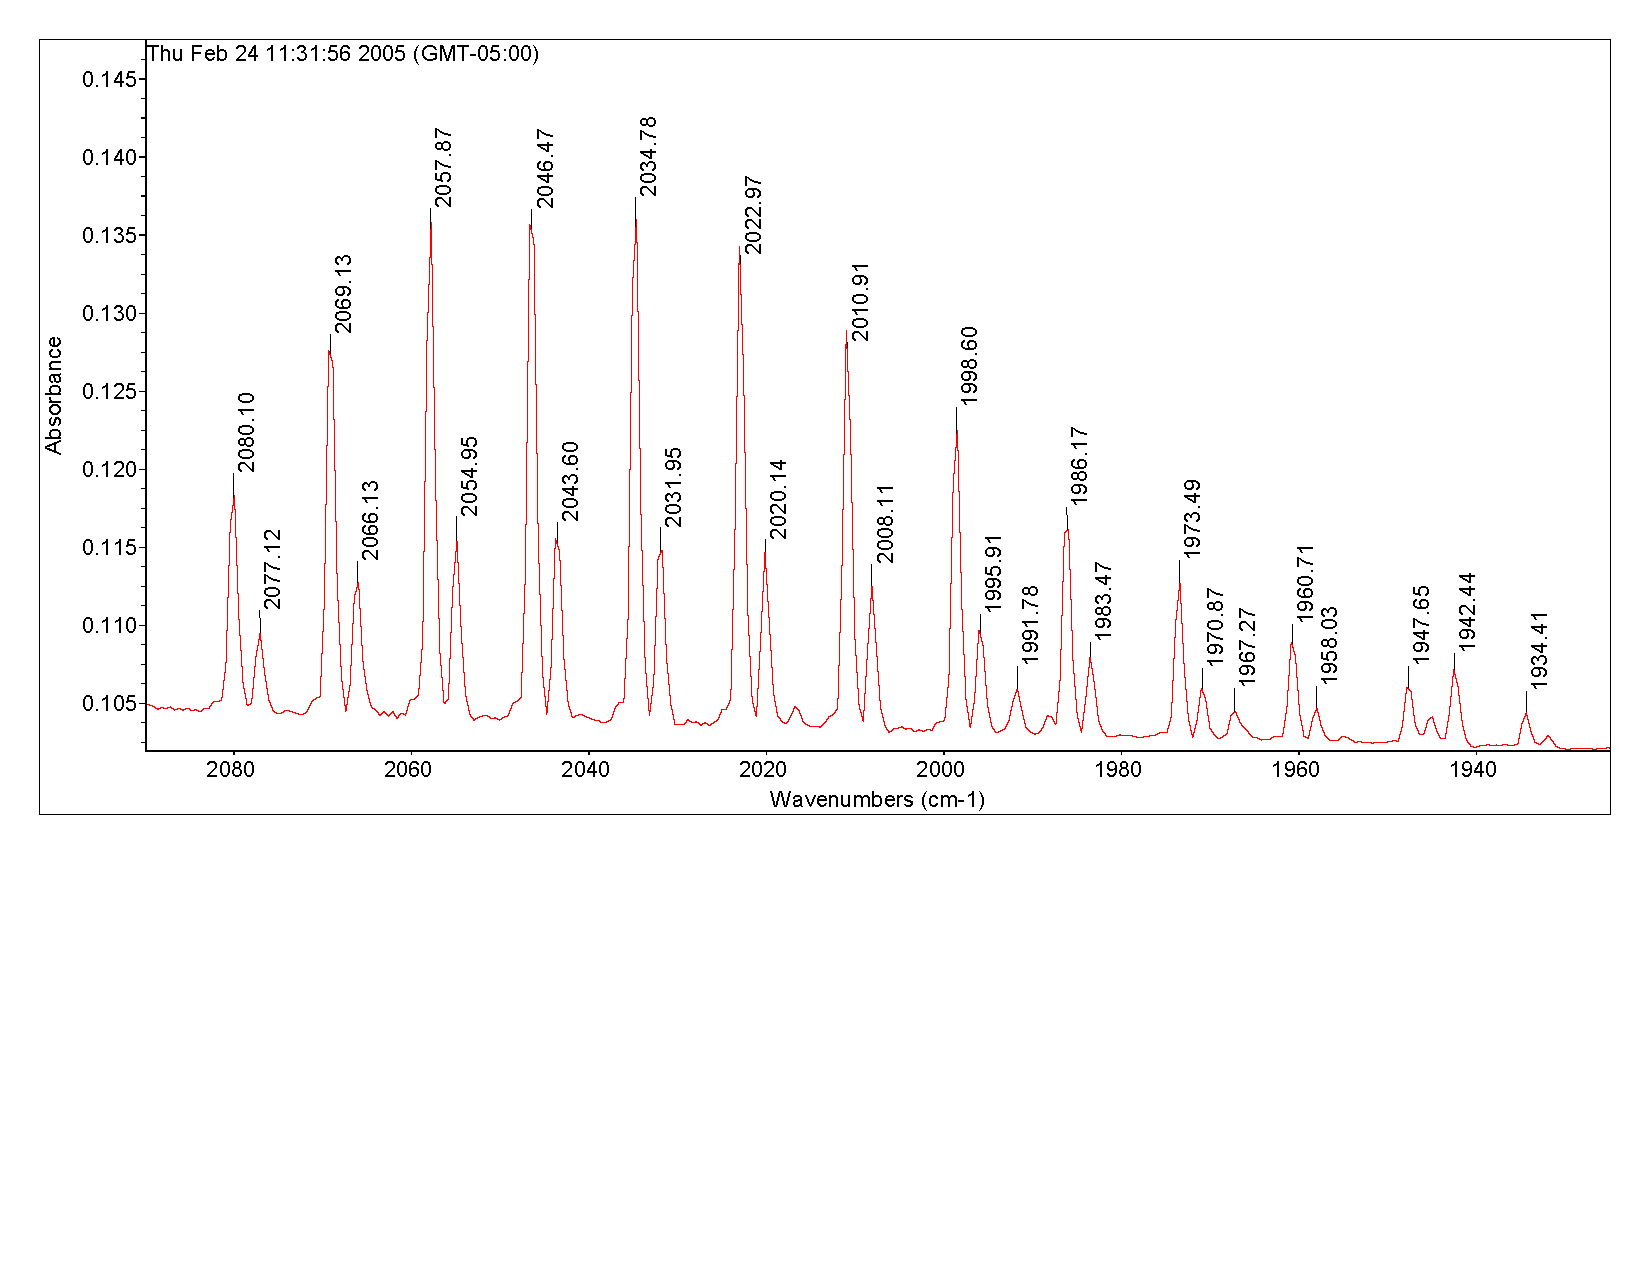
\includegraphics[width=\linewidth]{experimental_data/DCl_Right_clean.pdf}
        \caption{P-branch of D\(^{35}\)Cl}
    \end{subfigure}
    \hfill
    \begin{subfigure}{0.48\textwidth}
        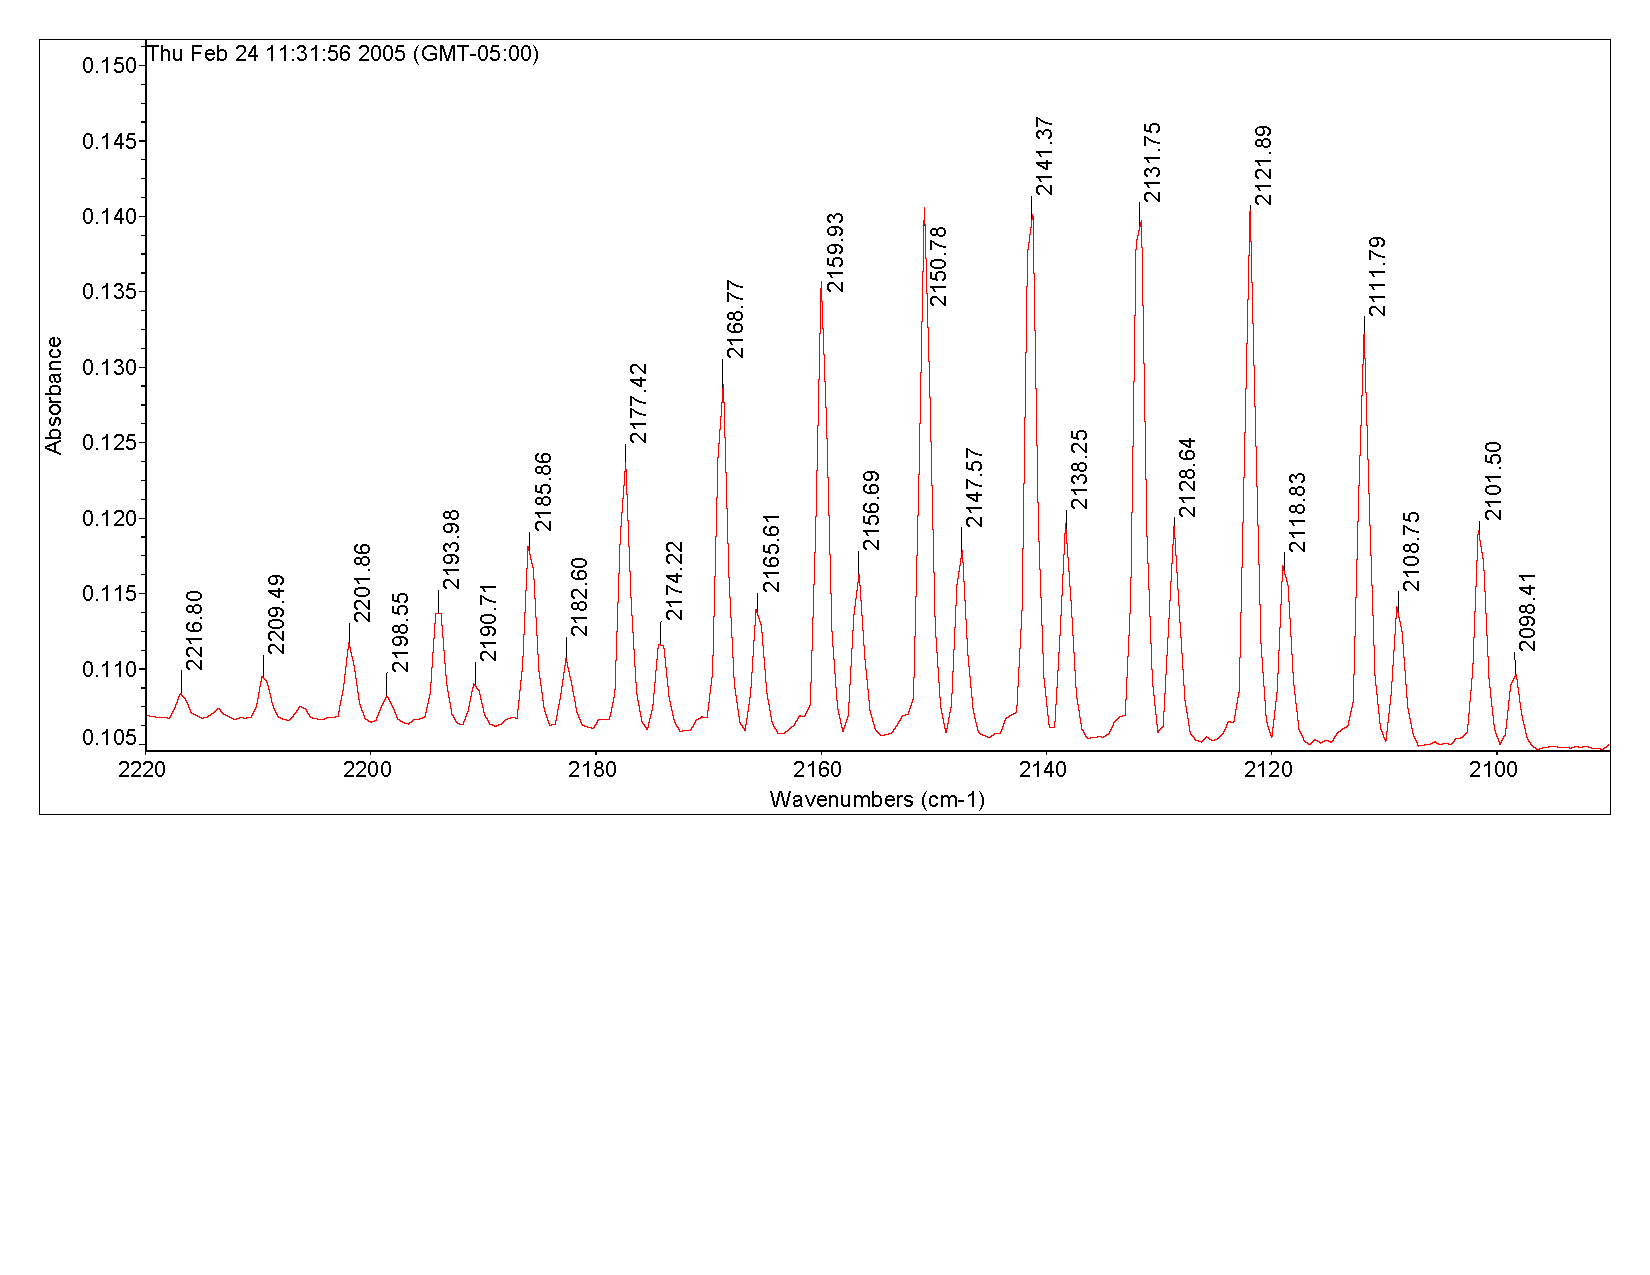
\includegraphics[width=\linewidth]{experimental_data/DCl_Left_clean.pdf}
        \caption{R-branch of D\(^{35}\)Cl}
    \end{subfigure}
    \caption{IR spectrum of D\(^{35}\)Cl.}
\end{figure}


The assigned peak positions are listed in Appendix. The linear regressions results with these data are used to calculate specific properties and presented here.

\begin{figure}[htbp]
    \centering
    \begin{subfigure}{0.48\textwidth}
        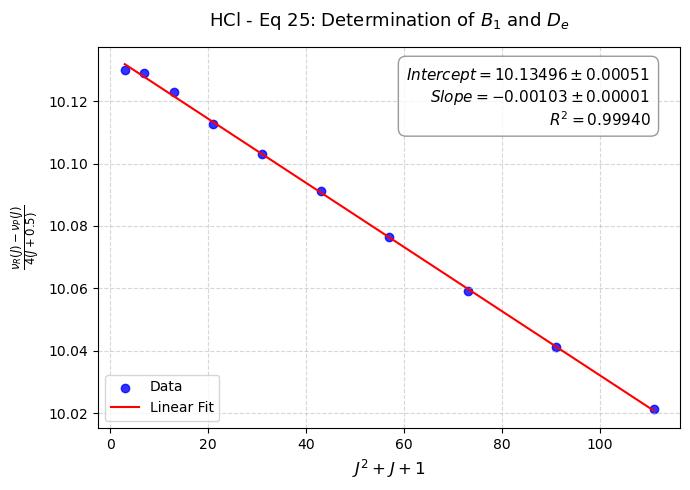
\includegraphics[width=\linewidth]{plot/HCl_eq25.png}
        \caption{H\(^{35}\)Cl, Eq.~(25).}
    \end{subfigure}
    \hfill
    \begin{subfigure}{0.48\textwidth}
        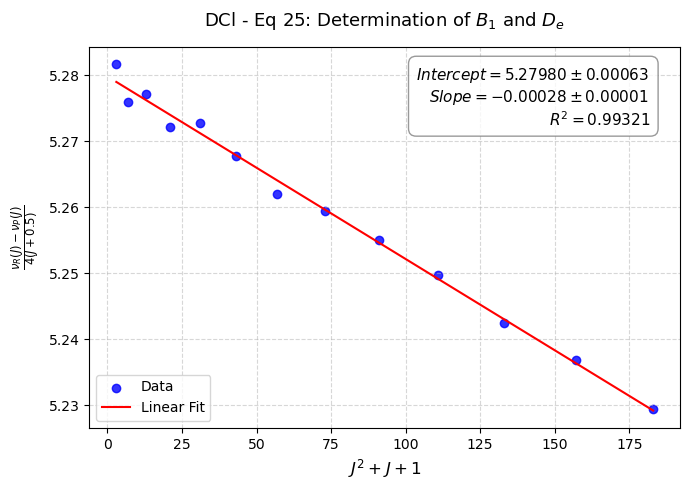
\includegraphics[width=\linewidth]{plot/DCl_eq25.png}
        \caption{D\(^{35}\)Cl, Eq.~(25).}
    \end{subfigure}
    \caption{Regression plots used to determine \(B_1\) and \(D_e\).}
\end{figure}

\begin{figure}[htbp]
    \centering
    \begin{subfigure}{0.48\textwidth}
        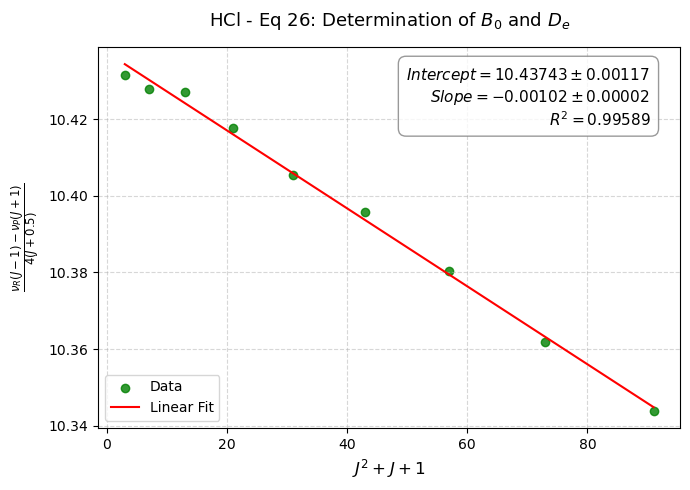
\includegraphics[width=\linewidth]{plot/HCl_eq26.png}
        \caption{H\(^{35}\)Cl, Eq.~(26).}
    \end{subfigure}
    \hfill
    \begin{subfigure}{0.48\textwidth}
        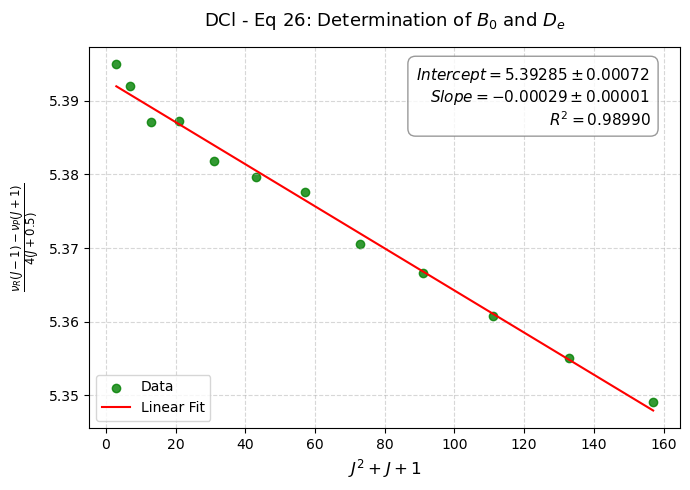
\includegraphics[width=\linewidth]{plot/DCl_eq26.png}
        \caption{D\(^{35}\)Cl, Eq.~(26).}
    \end{subfigure}
    \caption{Regression plots used to determine \(B_0\) and \(D_e\).}
\end{figure}

\begin{figure}[htbp]
    \centering
    \begin{subfigure}{0.48\textwidth}
        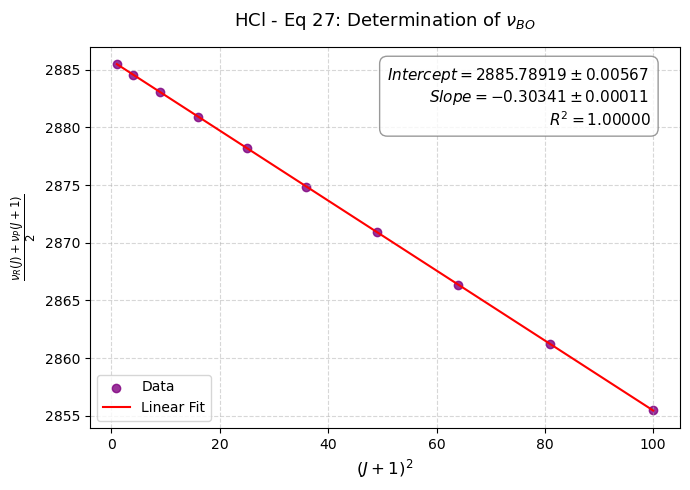
\includegraphics[width=\linewidth]{plot/HCl_eq27.png}
        \caption{H\(^{35}\)Cl, Eq.~(27).}
    \end{subfigure}
    \hfill
    \begin{subfigure}{0.48\textwidth}
        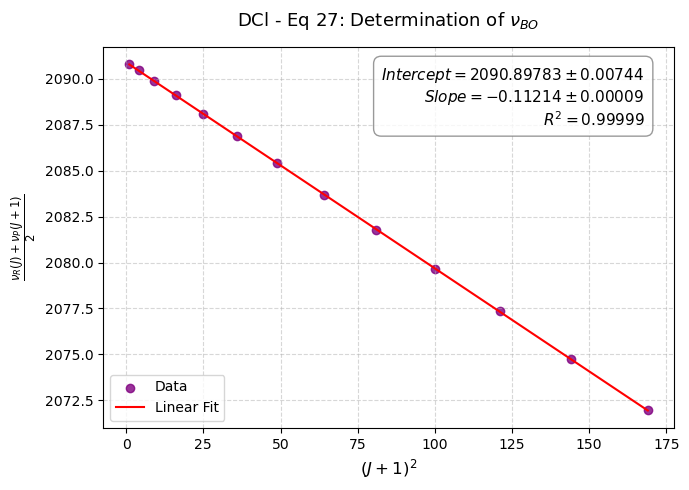
\includegraphics[width=\linewidth]{plot/DCl_eq27.png}
        \caption{D\(^{35}\)Cl, Eq.~(27).}
    \end{subfigure}
    \caption{Regression plots used to determine the band origin and \((B_1-B_0)\).}
\end{figure}

\begin{figure}[htbp]
    \centering
    \begin{subfigure}{0.48\textwidth}
        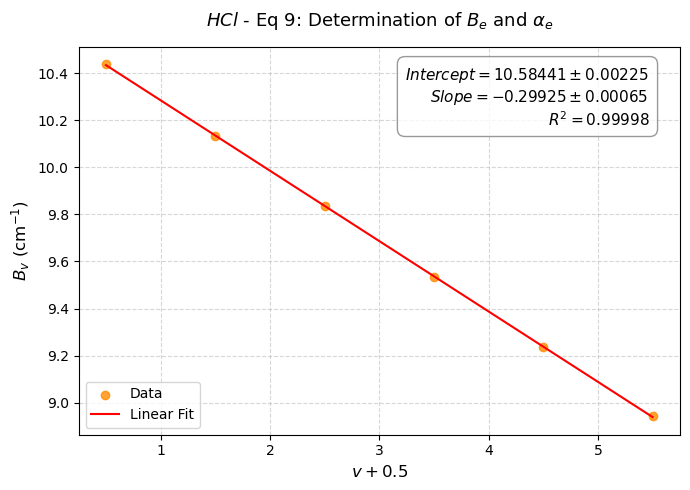
\includegraphics[width=\linewidth]{plot/HCl_eq9.png}
        \caption{H\(^{35}\)Cl, Eq.~(9).}
    \end{subfigure}
    \hfill
    \begin{subfigure}{0.48\textwidth}
        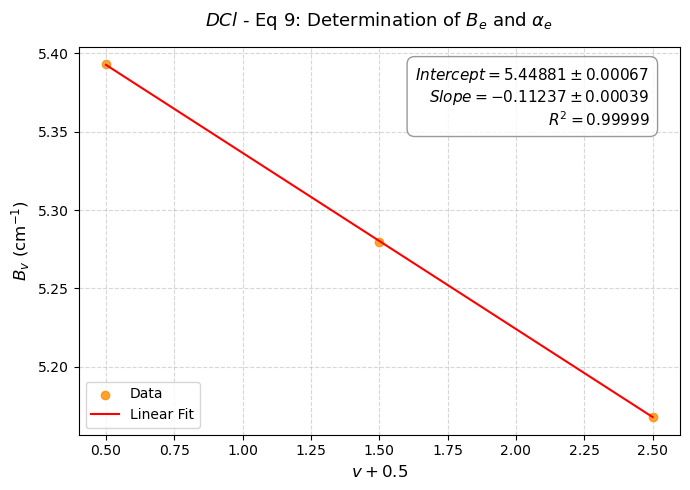
\includegraphics[width=\linewidth]{plot/DCl_eq9.png}
        \caption{D\(^{35}\)Cl, Eq.~(9).}
    \end{subfigure}
    \caption{Regression plots used to determine \(B_e\) and \(\alpha_e\).}
\end{figure}

\begin{figure}[htbp]
    \centering
    \begin{subfigure}{0.48\textwidth}
        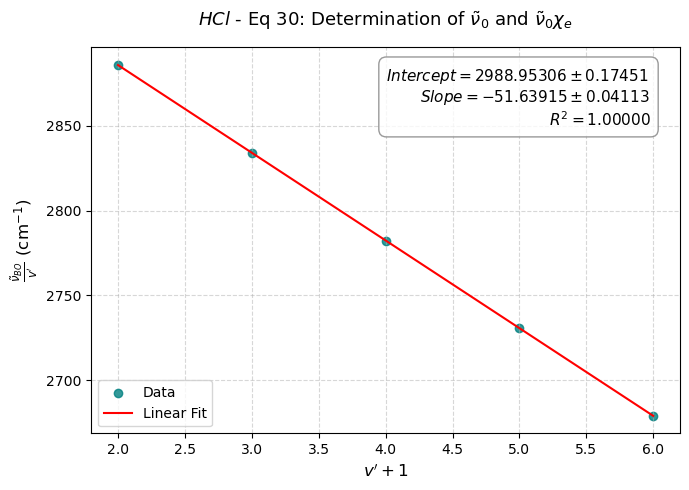
\includegraphics[width=\linewidth]{plot/HCl_eq30.png}
        \caption{H\(^{35}\)Cl, Eq.~(30).}
    \end{subfigure}
    \hfill
    \begin{subfigure}{0.48\textwidth}
        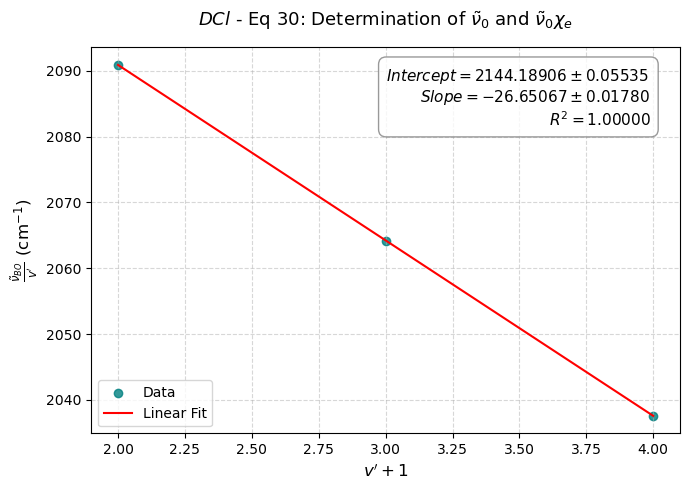
\includegraphics[width=\linewidth]{plot/DCl_eq30.png}
        \caption{D\(^{35}\)Cl, Eq.~(30).}
    \end{subfigure}
    \caption{Regression plots used to determine \(\tilde{\nu}_0\) and \(\tilde{\nu}_0\chi_e\).}
\end{figure}


The experimentally determined spectroscopic constants are summarized in Tables~\ref{tab:hcl_constants} and \ref{tab:dcl_constants}. The band origin \(\tilde{\nu}_{BO}\) was taken from the intercept of Eq.~(27), while the constants \(B_e\) and \(\alpha_e\) were obtained from the intercept and magnitude of the slope of Eq.~(9). Likewise, the intercept and slope magnitude of Eq.~(30) gave \(\tilde{\nu}_0\) and \(\tilde{\nu}_0\chi_e\), respectively.

\begin{table}[htbp]
\centering
\small
\caption{Experimental and literature spectroscopic constants for \(\mathrm{H}^{35}\mathrm{Cl}\).}
\label{tab:hcl_constants}
\begin{adjustbox}{max width=\linewidth}
\begin{tabular}{lccc}
\toprule
Parameter & Experimental value & Literature value & Error rate (\%) \\
\midrule
\(B_1\) (\(\mathrm{cm}^{-1}\)) & \(10.13496 \pm 0.00051\) & \(10.136223\) & \(0.01246\) \\
\(B_0\) (\(\mathrm{cm}^{-1}\)) & \(10.43743 \pm 0.00117\) & \(10.440254\) & \(0.02705\) \\
\(D_e^{25}\) (\(\times 10^{-4}\ \mathrm{cm}^{-1}\))& \(5.15000 \pm 0.05000\)& \(5.32019\) & \(3.19895\) \\
\(D_e^{26}\) (\(\times 10^{-4}\ \mathrm{cm}^{-1}\))& \(5.10000 \pm 0.10000\)& \(5.32019\) & \(4.13876\) \\
Averaged \(D_e\) (\(\times 10^{-4}\ \mathrm{cm}^{-1}\))& \(5.12500 \pm 0.05600\)& \(5.32019\) & \(3.66885\) \\
\(\tilde{\nu}_{BO}\) (\(\mathrm{cm}^{-1}\)) & \(2885.78919 \pm 0.00567\) & \(2885.97750\) & \(0.00652\) \\
\(B_e\) (\(\mathrm{cm}^{-1}\)) & \(10.58441 \pm 0.00225\) & \(10.593404\) & \(0.08490\) \\
\(\alpha_e\) (\(\mathrm{cm}^{-1}\)) & \(0.29925 \pm 0.00065\) & \(0.307139\) & \(2.56854\) \\
\(\tilde{\nu}_{0}\) (\(\mathrm{cm}^{-1}\)) & \(2988.95306 \pm 0.17451\) & \(2990.97424\) & \(0.06758\) \\
\(\tilde{\nu}_{0}\chi_e\) (\(\mathrm{cm}^{-1}\)) & \(51.63915 \pm 0.04113\) & \(52.84579\) & \(2.28332\) \\
\bottomrule
\end{tabular}
\end{adjustbox}
\end{table}

\begin{table}[htbp]
\centering
\small
\caption{Experimental and literature spectroscopic constants for \(\mathrm{D}^{35}\mathrm{Cl}\).}
\label{tab:dcl_constants}
\begin{adjustbox}{max width=\linewidth}
\begin{tabular}{lccc}
\toprule
Parameter & Experimental value & Literature value & Error rate (\%) \\
\midrule
\(B_1\) (\(\mathrm{cm}^{-1}\)) & \(5.27980 \pm 0.00063\) & \(5.279816\) & \(0.00030\) \\
\(B_0\) (\(\mathrm{cm}^{-1}\)) & \(5.39285 \pm 0.00072\) & \(5.392261\) & \(0.01092\) \\
\(D_e^{(25)}\) (\(\times 10^{-4}\ \mathrm{cm}^{-1}\)) & \(1.40 \pm 0.05\) & \(1.40000\) & \(0.00000\) \\
\(D_e^{(26)}\) (\(\times 10^{-4}\ \mathrm{cm}^{-1}\)) & \(1.45 \pm 0.05\) & \(1.40000\) & \(3.57143\) \\
Averaged \(D_e\) (\(\times 10^{-4}\ \mathrm{cm}^{-1}\))& \(1.425 \pm 0.035\) & \(1.40000\) & \(1.78571\) \\
\(\tilde{\nu}_{BO}\) (\(\mathrm{cm}^{-1}\)) & \(2090.89783 \pm 0.00744\) & \(2091.06130\) & \(0.00782\) \\
\(B_e\) (\(\mathrm{cm}^{-1}\)) & \(5.44881 \pm 0.00067\) & \(5.448794\) & \(0.00029\) \\
\(\alpha_e\) (\(\mathrm{cm}^{-1}\)) & \(0.11237 \pm 0.00039\) & \(0.113291\) & \(0.81295\) \\
\(\tilde{\nu}_{0}\) (\(\mathrm{cm}^{-1}\)) & \(2144.18906 \pm 0.05535\) & \(2145.16300\) & \(0.04540\) \\
\(\tilde{\nu}_{0}\chi_e\) (\(\mathrm{cm}^{-1}\)) & \(26.65067 \pm 0.01780\) & \(27.18252\) & \(1.95659\) \\
\bottomrule
\end{tabular}
\end{adjustbox}
\end{table}

\begin{table}[htbp]
\centering
\small
\caption{Derived structural parameters and comparison with literature values.}
\label{tab:derived_parameters}
\begin{adjustbox}{max width=\linewidth}
\begin{tabular}{llccc}
\toprule
Species & Parameter & Experimental value & Literature value\cite{sime1990lit_all,herzberg2013bond_lit,lide2002constant_lit} & Error rate (\%) \\
\midrule
\(\mathrm{H}^{35}\mathrm{Cl}\) & \(\tilde{\nu}_e\) (\(\mathrm{cm}^{-1}\)) & \(3092.23136 \pm 0.19293\) & --- & --- \\
\(\mathrm{H}^{35}\mathrm{Cl}\) & \(r_e\) (\(\text{Ang}\))& \(1.27509 \pm 0.00014\) & \(1.27460\) & \(0.03844\) \\
\(\mathrm{H}^{35}\mathrm{Cl}\) & \(k\) (\(\mathrm{N\,m^{-1}}\)) & \(551.87366 \pm 0.06886\)& \(516\) & \(6.95226\)\\
\(\mathrm{D}^{35}\mathrm{Cl}\) & \(\tilde{\nu}_e\) (\(\mathrm{cm}^{-1}\)) & \(2197.49040 \pm 0.06581\) & --- & --- \\
\(\mathrm{D}^{35}\mathrm{Cl}\) & \(r_e\) (\(\text{Ang}\))& \(1.27458 \pm 0.00008\) & \(1.274\) & \(0.04553\) \\
\(\mathrm{D}^{35}\mathrm{Cl}\) & \(k\) (\(\mathrm{N\,m^{-1}}\)) & \(541.83065 \pm 0.03540\)& \(516\) & \(5.00594\)\\
\bottomrule
\end{tabular}
\end{adjustbox}
\end{table}

\newpage
\section*{Discussion}
The experimental results show that the rotational and vibrational constants obtained from the FTIR spectra are basically consistent with literature values\cite{lide2002constant_lit,herzberg2013bond_lit,sime1990lit_all}. The relative errors observed for \(B_1\), \(B_0\), \(B_e\), and the band origins were all below about 0.1\% for both isotope compounds. It indicates that the line assignments were reliable and that the rotational structure was measured accurately. The larger discrepancies appeared in \(\alpha_e\), \(\tilde{\nu}_0\chi_e\), and the derived force constants. Those quantities depend more strongly on small differences of fitted quantities or on the overtone-based extrapolation, so they are more sensitive to errors in the experimental line positions.

The bond lengths agreed well with literature values. The relative errors were $0.03844\%$ for H\(^{35}\)Cl and $0.04553\%$ for D\(^{35}\)Cl. While the force constants were higher than the literature value of \SI{516}{N\,m^{-1}} by $6.95226\%$ for H\(^{35}\)Cl and $5.00594\%$ for D\(^{35}\)Cl. The most likely sources of this systematic overestimation are uncertainty in peak picking and the propagation of small fitting errors into \(\tilde{\nu}_e\) and then into \(k\).

In the spectrum, there is no \(\tilde{\nu}_P(0)\) line because the P branch corresponds to \(\Delta J=-1\). If the lower state has \(J''=0\), the upper state would need to have \(J'=-1\), which is impossible because rotational quantum numbers cannot be negative. So, the first allowed P-branch transition is \(P(1)\), while the first R-branch transition is \(R(0)\).

In principle, the equilibrium bond lengths of HCl and DCl should be highly similar or even the same. Isotopic substitution changes the nuclear masses, the rotational and vibrational spacings, but it does not quite change the electronic potential energy curve. Experimentally, this expectation was confirmed: \(r_e(\mathrm{HCl})=1.27509\pm0.00014\ \text{Ang}\) and \(r_e(\mathrm{DCl})=1.27458\pm0.00008\ \text{Ang}\), differing by only \SI{0.00051}{\angstrom}.

Moreover, the bond force constants of HCl and DCl should also be essentially the same or highly similar because both isotope compounds share the same bonding potential. The result values, \(551.87366 \pm 0.06886\) and \(541.83065 \pm 0.03540\ \mathrm{N\,m^{-1}}\), have very small compared with the overall systematic error relative to literature. Ignoring anharmonicity, the tritium chloride frequency may be estimated from the reduced-mass dependence \(\tilde{\nu}\propto \mu^{-1/2}\). Using our HCl results gives \(\tilde{\nu}(\mathrm{TCl})\approx 1836\) $\mathrm{cm^{-1}}$. The equilibrium bond length in tritium chloride should be essentially unchanged from those of HCl and DCl, so a reasonable estimate is \(r_e(\mathrm{TCl})\approx 1.274\ \text{Ang}\).

\section*{Conclusion}
In summary, in this experiment, the FTIR spectra provided accurate rotational constants and band origins for H\(^{35}\)Cl and D\(^{35}\)Cl, and the isotope trends agreed with reduced-mass expectations. The bond length and elastic constant are also well determined with calcualtions.


\newpage
% References section 
% Must follow American Chemical Society (ACS) format. 
\bibliographystyle{achemso} % Uses the ACS formatting style
\bibliography{references} % Ensure you create a references.bib file in your directory

\newpage
\section*{Appendix}
\addcontentsline{toc}{section}{Appendix}
% Include supplementary material (raw output, sample calculations) 
The raw data and corresponding analysis script are available on \href{https://github.com/EasonShi0624/26Spring-PChemLab/tree/main/Lab_4_Vibrational-Rotational_Spectra_of_Diatomic_Molecules}{\textcolor{RoyalBlue}{GitHub} \faGithub}

\begin{figure}[htbp]
    \centering
    
\includegraphics[width=0.7\linewidth, keepaspectratio, page=1]{Lab Computation.pdf}
    \caption{Computations of Values and Error Analysis (Page 1)}
    \label{fig:lab_comp_p1}
\end{figure}

\begin{figure}[htbp]
    \centering
    
\includegraphics[width=0.9\linewidth, keepaspectratio, page=2]{Lab Computation.pdf}
    \caption{Computations of Values and Error Analysis (Page 2)}
    \label{fig:lab_comp_p1}
\end{figure}


\begin{figure}[htbp]
    \centering
    
\includegraphics[width=0.9\linewidth, keepaspectratio, page=3]{Lab Computation.pdf}
    \caption{Computations of Values and Error Analysis (Page 3)}
    \label{fig:lab_comp_p1}
\end{figure}


\begin{figure}[htbp]
    \centering
    
\includegraphics[width=0.9\linewidth, keepaspectratio, page=4]{Lab Computation.pdf}
    \caption{Computations of Values and Error Analysis (Page 4)}
    \label{fig:lab_comp_p1}
\end{figure}


\begin{figure}[htbp]
    \centering
    
\includegraphics[width=0.9\linewidth, keepaspectratio, page=5]{Lab Computation.pdf}
    \caption{Computations of Values and Error Analysis (Page 5)}
    \label{fig:lab_comp_p1}
\end{figure}

\begin{figure}[htbp]
    \centering
    
\includegraphics[width=0.9\linewidth, keepaspectratio, page=6]{Lab Computation.pdf}
    \caption{Computations of Values and Error Analysis (Page 6)}
    \label{fig:lab_comp_p1}
\end{figure}


\begin{figure}[htbp]
    \centering
    
\includegraphics[width=0.9\linewidth, keepaspectratio, page=7]{Lab Computation.pdf}
    \caption{Computations of Values and Error Analysis (Page 7)}
    \label{fig:lab_comp_p1}
\end{figure}


\begin{figure}[htbp]
    \centering
    
\includegraphics[width=0.9\linewidth, keepaspectratio, page=8]{Lab Computation.pdf}
    \caption{Computations of Values and Error Analysis (Page 8)}
    \label{fig:lab_comp_p1}
\end{figure}

\begin{figure}[htbp]
    \centering
    
\includegraphics[width=0.9\linewidth, keepaspectratio, page=9]{Lab Computation.pdf}
    \caption{Computations of Values and Error Analysis (Page 9)}
    \label{fig:lab_comp_p1}
\end{figure}



\begin{figure}[htbp]
    \centering
    
\includegraphics[width=0.9\linewidth, keepaspectratio, page=1]{lab_note.pdf}
    \caption{Raw Lab Notes}
    \label{fig:lab_notes}
\end{figure}


\end{document}